%! TeX program = lualatex
\documentclass[12pt,a4paper]{article}

\usepackage[nil]{babel}
\usepackage{unicode-math}
\usepackage[svgnames]{xcolor}
\usepackage{lmodern}
\usepackage{graphicx}
\usepackage{wrapfig}
\usepackage{float}
\usepackage{parskip}
\usepackage{xurl}
\usepackage{hyperref}
\usepackage{fullpage}
\usepackage[font=small,labelfont=bf,justification=centering]{caption}

\babelprovide[import=el, main, onchar=ids fonts]{greek} % can also do import=el-polyton
\babelprovide[import, onchar=ids fonts]{english}

\babelfont{rm}
          [Language=Default]{Liberation Sans}
\babelfont[english]{rm}
          [Language=Default]{Liberation Sans}
\babelfont{sf}
          [Language=Default]{Liberation Sans}
\babelfont{tt}
          [Language=Default]{Liberation Sans}

\renewcommand{\thesubsection}{\thesection.\alph{subsection}}
\setlength{\emergencystretch}{3em}

%Enter Title Here
\title{Εργασία Υπολογιστική Νοημοσύνη\\Μέρος Β}
\author{Γρηγόρης Καπαδούκας (ΑΜ: 1072484)}

\begin{document}
\maketitle

\setcounter{section}{-1}
\section{Περιβάλλον Εργασίας - Σύνδεσμος GitHub με Κώδικα}
Για την διεκπεραίωση αυτής της εργασίας έχω επιλέξει να χρησιμοποιήσω γλώσσα προγραμματισμού Python μαζί τις βιβλιοθήκες PyGAD για την υλοποίηση του γενετικού αλγορίθμου και TensorFlow (κυρίως το API της, το Keras) για τον σχεδιασμό και την εκπαίδευση του νευρωνικού δικτύου από το μέρος Α. Επίσης χρησιμοποιώ Pandas, NumPy, SciPy, Matplotlib και Scikit-Learn με σκοπό τον χειρισμό του CSV αρχείου, της προεπεξεργασίας και άλλων μαθηματικών διαδικασιών.

Ο κώδικας που γράφτηκε για την εργασία βρίσκεται στο repository στον παρακάτω σύνδεσμο:

\textcolor{blue}{\href{https://github.com/GregKapadoukas/University-Computational-Intelligence-Project-B}{https://github.com/GregKapadoukas/University-Computational-Intelligenc\\e-Project-B}}

Στο repository αυτό συμπεριλαμβάνω και το αρχείο 'environment.yml' το οποίο μπορεί να χρησιμοποιηθεί με χρήση του εργαλείου conda για να δημιουργηθεί πανομοιότυπο Python virtual environment με αυτό που χρησιμοποίησα για τη συγγραφή και εκτέλεση του κώδικα. Βέβαια για χρήση της βιβλιοθήκης TensorFlow απαιτούνται επιπλέον configuration βήματα, που αναλύονται στην εξής σελίδα:
\textcolor{blue}{\href{https://www.tensorflow.org/install/pip}{https://www.tensorflow.org/install/pip}}

\section{Σχεδιασμός Γενετικού Αλγόριθμου}

\subsection{Κωδικοποίηση}

Παρατηρώντας τα δεδομένα του dataset βλέπουμε ότι για οι αισθητήρες είναι συνολικά 4, και τα δεδομένα για κάθε αισθητήρα είναι 3 σε κάθε περίπτωση, δίνοντας συνολικά 12 πραγματικές τιμές στο εύρος [-702, 533] (υποθέτοντας πως οι αισθητήρες παράγουν τιμές στο ίδιο εύρος και πως έχουν παρατηρηθεί τα άκρα των πιθανών τιμών στις μετρήσεις του dataset. Στον κώδικα χρησιμοποιώντας τη συνάρτηση .describe() του Pandas εμφανίζουμε τη μέγιστη και ελάχιστη τιμή για κάθε αισθητήρα που παρατηρήθηκε στο dataset).

Λόγω του συνδυασμού του μεγάλου πλήθους τιμών που χρησιμοποιούνται για την αναπαράσταση της κλάσης κίνησης και του μεγάλου εύρους στο οποίο ανήκουν οι τιμές αυτές, αποφάσισα να χρησιμοποιήσω float-valued encoding, σε συνδυασμό με MinMax scaling στο εύρος [0,1].

Άρα η λύση που προσεγγίζουμε καθώς και κάθε χρωμόσωμα, θα αποτελούνται από ένα πίνακα πραγματικών αριθμών στο εύρος [0,1] μεγέθους 12. Εννοείται πως όταν βρεθεί η βέλτιστη λύση θα κάνουμε inverse MinMax scaling ώστε να επαναφερθούν οι τιμές στο εύρος [-702, 533]. 

\subsection{Πλεονάζουσες Τιμές}

Αρχικά με τη χρήση του float-valued encoding, κανονικά μπορεί να υπάρξει πιθανότητα να προκύψουν πλεονάζοντες τιμές, δηλαδή τιμές εκτός του εύρους των τιμών των αισθητήρων. Μάλιστα λόγω της χρήσης του MinMax scaling που αναφέρθηκε, το εύρος πλέον στο οποίο πρέπει να περιέχονται όλες οι τιμές των γονιδίων σε κάθε χρωμόσωμα που παράγει ο γενετικός αλγόριθμος είναι το [0,1], στο οποίο με μετέπειτα χρήση inverse scaling θα οδηγήσει στα μη κανονικοποιημένα αποτελέσματα στο εύρος των τιμών του αισθητήρων, ώστε να γίνει η σύγκριση με τους μέσους όρους των τιμών των αισθητήρων για την κλάση 'sitting' από τα δεδομένα του dataset.

Με σκοπό να αποφύγουμε τις πλεονάζουσες τιμές τελείως αρκεί να μελετήσουμε τα ενδεχόμενα αρχικά για τον τελεστή της διασταύρωσης και μετά για τον τελεστή της μετάλλαξης. Σχετικά με τον τελεστή της διασταύρωσης δεν υπάρχει περίπτωση να παραχθεί τιμή εκτός του εύρους [0,1], εφόσον με float-valued encoding απλά ανταλλάσσονται γονίδια μεταξύ των χρωμοσωμάτων (στη προσέγγιση που επέλεξα).

Σχετικά με τον τελεστή μετάλλαξης, λόγω του τελεστή της τυχαίας μετάλλαξης που επιλέγω να χρησιμοποιήσω και αναλύω αργότερα και της αντικατάστασης των γονιδίων με τις τυχαίες τιμές και οι τυχαίες τιμές που παράγονται βρίσκονται στο εύρος [0,1], δεν υπάρχει ανάγκη για παραπάνω αντιμετώπιση.

Άρα καταλήγω πως ο συνδυασμός του encoding που επέλεξα μαζί με τους τελεστές δεν οδηγούν ποτέ σε πλεονάζοντες τιμές.

\subsection{Αρχικός Πληθυσμός}

Για τη δημιουργία του αρχικού πληθυσμού δοκίμασα δύο προσεγγίσεις: 

\begin{itemize}
    \item \textbf{Τυχαία Αρχικοποίηση:} Η πρώτη προσέγγιση είναι να χρησιμοποιήσω τυχαίες τιμές που προέρχονται από ομοιόμορφη κατανομή με εύρος τιμών [0,1]. 

    \item \textbf{Χρήση Latin Hypercube Sampling:} Η δεύτερη προσέγγιση χρησιμοποιεί Latin Hypercube Sampling, όπου αρχικά το εύρος της κάθε τιμής για γονίδιο, δηλαδή το [0,1] σε αυτή τη περίπτωση, χωρίζεται σε όσα μέρη είναι και ο αριθμός των χρωμοσωμάτων στον αρχικό πληθυσμό. Έπειτα για κάθε χρωμόσωμα γίνεται τυχαία επιλογή για κάθε γονίδιο ένα από τα μέρη του πεδίου που προέκυψαν, και διαλέγεται μια τυχαία τιμή από ομοιόμορφη κατανομή στο εύρος αυτό. Η διαδικασία αυτή γίνεται με τρόπο ώστε κάθε μέρος του χωρισμένου πεδίου ορισμού να επιλεχθεί μια φορά για το γονίδιο αυτό στο σύνολο του πληθυσμού.
\end{itemize}

Θεωρητικά η προσέγγιση του Latin Hypercube Sampling είναι η καλύτερη των δύο, επειδή εξασφαλίζει ότι ο αρχικός πληθυσμός θα έχει χρωμοσώματα που θα αναπαριστούν καλύτερα όλο το εύρος πιθανών τιμών, προσθέτοντας βέβαια κάποια επιπλέον πολυπλοκότητα για την αρχικοποίηση.

Στη πράξη όμως δοκιμάζοντας και τις δύο προσεγγίσεις, η διαφορά στα αποτελέσματα για αυτό το πρόβλημα ήταν αμελητέο, αλλά επέλεξα και πάλι το Latin Hypercube Sampling για την θεωρητική ανωτερότητά του σαν προσέγγιση αρχικοποίησης αρχικού πληθυσμού.

Σημειώνω ότι λόγω του εύρους [0,1] που επιλέχθηκε, τα χρωμοσώματα του πληθυσμού είναι ήδη κανονικοποιημένα και μετά από inverse MinMax scaling θα ανήκουν στο εύρος των πιθανών τιμών που θα μπορούσαν να έχουν οι αισθητήρες στο ρομπότ.

\subsection{Υπολογισμός Ομοιότητας}

Αρχικά, με σκοπό το σχολιασμό της καταλληλότητας της ομοιότητας συνημιτόνου σε σχέση με τις άλλες μετρικές ομοιότητας, θα αναφέρω κάποια βασικά ζητήματα για τις μετρικές:

Η ευκλείδεια απόσταση και η απόσταση Manhattan, χρησιμοποιούν την δεύτερη και πρώτη νόρμα αντίστοιχα, με σκοπό να υπολογίσουν την απόσταση. Το προτέρημα της ευκλείδειας απόστασης είναι ότι για μεγαλύτερη διαφορά μεταξύ των τιμών των γονιδίων, η απόσταση γίνεται μεγαλύτερη με τετραγωνικό ρυθμό, οπότε δημιουργείται μεγαλύτερη αύξηση στη τελική απόσταση, σε σχέση με την απόσταση Manhattan, όπου η απόσταση αυξάνεται με γραμμικό ρυθμό όσο αυξάνεται η διαφορά στα γονίδια.

\begin{itemize}
    \item \textbf{Ευκλείδεια και Manhattan Αποστάσεις:} Οπότε αν ήθελα να χρησιμοποιήσω ευκλείδεια ή Manhattan απόσταση ως συνάρτηση καταλληλότητας, θα έπρεπε να αυτό να γίνεται σε μια σχέση όπου όσο μειώνεται η απόσταση κάθε φορά, τόσο να αυξάνεται η συνάρτηση καταλληλότητας, εφόσον οι γενετικοί αλγόριθμοι προσπαθούν να αυξήσουν όσο δυνατό τη συνάρτηση καταλληλότητας ενώ εγώ θέλω να ελαχιστοποιήσω την απόσταση.

    \item \textbf{Ομοιότητα Συνημιτόνου:} Η ομοιότητα συνημιτόνου από την άλλη υπολογίζει τη τιμή του συνημιτόνου της γωνίας που προκύπτουν μεταξύ των δύο διανυσμάτων από τα οποία υπολογίζεται η μετρική. Έχει εύρος πιθανών τιμών από 0 έως 1 (για μη αρνητικά διανύσματα όπως εδώ, αλλιώς από -1 έως 1 αν υπάρχουν και αρνητικά διανύσματα) και για πολλαπλάσια των διανυσμάτων που ελέγχονται δεν αλλάζει η γωνία, οπότε δεν αλλάζει και η απόσταση συνημιτόνου. Αυτή η ιδιότητα ανάλογα το πρόβλημα και τη προσέγγιση της λύσης που εφαρμόζεται, μπορεί να συμβάλλει ή να στερήσει την απόδοση της λύσης.
        
    \item \textbf{Συσχέτιση Pearson:} Η συσχέτιση Pearson υπολογίζει τη συσχέτιση μεταξύ των τιμών του πρώτου γονιδίου σε σχέση με το δεύτερο γονίδιο, δηλαδή υπολογίζει αν παρατηρώντας μια νέα τιμή για το ένα γονίδιο, με πόση ακρίβεια μπορούμε να εξάγουμε συμπεράσματα για την τιμή του δεύτερου γονιδίου. Οι τιμές της συσχέτισης Pearson έχουν εύρος από -1, δηλαδή πλήρη αρνητική συσχέτιση, έως 1, δηλαδή πλήρη θετική συσχέτιση, με τιμή 0 να δείχνει καμία συσχέτιση. Η μετρική αυτή δεν είναι τόσο χρήσιμη σε αυτή τη περίπτωση, επειδή η συσχέτιση των γονιδίων κάθε φορά του γενετικού αλγορίθμου σε σχέση με τους μέσους όρους των τιμών του αισθητήρα δεν παρουσιάζει πληροφορία για τη κλάση κίνησης του ρομπότ.
\end{itemize}

Οπότε καταλήγουμε πως η ομοιότητα συνημιτόνου αυτομάτως είναι πιο κατάλληλη από την συσχέτιση Pearson, και ταυτόχρονα έχει ευκολότερη εφαρμογή στη συνάρτηση καταλληλότητας σε σχέση με την ευκλείδεια και Manhattan απόσταση, λόγω του επιθυμητού χαρακτηριστικού να αυξάνεται όσο πιο όμοια είναι τα δύο διανύσματα. 

Ταυτόχρονα επειδή οι τιμές των αισθητήρων του dataset προέρχονται από επιταχυνσιόμετρα, είναι πολύ πιθανό οι πολλαπλάσιες τιμές να ανήκουν κάθε φορά στην ίδια κλάση, κάτι που κάνει τη χρήση της ομοιότητας συνημιτόνου ακόμα πιο επιθυμητή.

\subsection{Συνάρτηση Καταλληλότητας}

\subsubsection{}

\textbf{Σημείωση:} Όλες οι παρακάτω πράξεις έχουν γίνει με τη προϋπόθεση ότι όλα τα διανύσματα είναι θετικά, οπότε η ομοιότητα συνημιτόνου κινείται στο εύρος [0, 1], εφόσον η προσέγγιση σχεδιασμού του ΓΑ που έχω κάνει μέχρι τώρα δεν οδηγεί ποτέ σε αρνητικά διανύσματα. Αν η προσέγγιση ήταν διαφορετική και υπήρχαν αρνητικά διανύσματα, τότε οι παρακάτω πράξεις δεν θα ίσχυαν.

Η θεωρητική μέγιστη τιμή της F είναι για μέγιστη ομοιότητα συνημιτόνου μεταξύ του $v$ και $t_s$, με μηδενική ομοιότητα μεταξύ του $v$ και όλων των $t_s$. Άρα με αντικατάσταση υπολογίζω:

\begin{center}
    $F(v)_\mathrm{max} = \frac{cos(v,t_s) + c(1-\frac{1}{4}\sum_{i\neq s}cos(v,t_i))}{1+c} \implies$

    $F(v)_\mathrm{max} = \frac{1 + c(1-\frac{1}{4}\cdot0)}{1+c} \implies$

    $F(v)_\mathrm{max} = \frac{1 + c(1-0)}{1+c} \implies$

    $F(v)_\mathrm{max} = \frac{1 + c}{1+c} \implies$

    $F(v)_\mathrm{max} = 1$
\end{center}

Στη πράξη όμως, μέχρι και το πραγματικό χρωμόσωμα με τη μεγαλύτερη εξ ορισμού καταλληλότητα, δεν έχει μηδενική ομοιότητα συνημιτόνου συγκριτικά με τις άλλες μέσες τιμές για τις άλλες κλάσεις κίνησης. Οπότε η μόνη περίπτωση στη πράξη να έχουμε τιμή $F(v) = 1$ είναι για $v = s$ καθώς και $c = 0$.

Ο υπολογισμός πραγματικής ελάχιστης τιμής στη περίπτωση αυτή είναι εξαιρετικά δύσκολη διαδικασία, και μπορεί μόνο να προσεγγιστεί, οπότε θα υπολογίσω μόνο τη θεωρητική ελάχιστη τιμή, για μηδενική ομοιότητα συνημιτόνου με το $s$ και τέλεια ομοιότητα με όλα τα $t_s$ (προφανώς κάτι που δεν θα συνέβαινε ποτέ στη πράξη). Άρα με αντικατάσταση υπολογίζω:

\begin{center}
    $F(v)_\mathrm{min} = \frac{cos(v,t_s) + c(1-\frac{1}{4}\sum_{i\neq s}cos(v,t_i))}{1+c} \implies$

    $F(v)_\mathrm{min} = \frac{0 + c(1-\frac{1}{4}\cdot1)}{1+c} \implies$

    $F(v)_\mathrm{min} = \frac{\frac{3}{4}\cdot c}{1+c} \implies$

    $F(v, c = 0)_\mathrm{min} = \frac{\frac{3}{4}\cdot 0}{1+0} \implies$

    $F(v)_\mathrm{min} = 0$
\end{center}

Οπότε παρατηρούμε ότι δεν υπάρχουν αρνητικές τιμές καταλληλότητας, εφόσον το θεωρητικό ελάχιστο είναι ίσο με 0. Ο τρόπος που τις αποφύγαμε ήταν μέσω της αποφυγής αρνητικών διανυσμάτων μέσω του MinMax scaling.

\subsubsection{}

Με βάση τις προδιαγραφές της εκφώνησης, η συνάρτηση καταλληλότητας πρέπει να οδηγεί σε υψηλές τιμές όταν τα γονίδια είναι κοντά στις μέσες τιμές των αισθητήρων για τη κατάσταση κίνησης 'sitting' και ταυτόχρονα να οδηγεί σε χαμηλότερες τιμές όταν τα γονίδια είναι κοντά στις μέσες τιμές των αισθητήρων για τις άλλες καταστάσεις. Από την συνάρτηση καταλληλότητας παρατηρούμε τα εξής:

\begin{center}
    $F(v) = \frac{cos(v,t_s) + c(1-\frac{1}{4}\sum_{i\neq s}cos(v,t_i))}{1+c} \implies$

    $F(v) = \frac{cos(v,t_s) + c - c\cdot\frac{1}{4}\sum_{i\neq s}cos(v,t_i)}{1+c} \implies$

    $F(v) = \frac{cos(v,t_s) + c}{1+c} - \frac{c\cdot\frac{1}{4}\sum_{i\neq s}cos(v,t_i)}{1+c}$
\end{center}

Οπότε όσο αυξάνεται το $cos(v,t_s)$, τόσο αυξάνεται το πρώτο φράγμα και το αποτέλεσμα, και όσο αυξάνονται τα $cos(v,t_i)$ τόσο αυξάνεται το δεύτερο φράγμα και μειώνεται το αποτέλεσμα. Η τιμή c ορίζει το ποσοστό συμβολής του δεύτερου φράγματος στο τελικό αποτέλεσμα.

Άρα η συνάρτηση αυτή έχει τα επιθυμητά χαρακτηριστικά και είναι κατάλληλη επιλογή για χρήση ως συνάρτηση καταλληλότητας.

\subsubsection{}

Εφόσον η τιμή της σταθεράς c παίζει το ρόλο ενός ποσοστού που συμβάλλει η ελαχιστοποίηση της ομοιότητας με τις άλλες καταστάσεις στην έξοδο της συνάρτησης καταλληλότητας σε σχέση με την μεγιστοποίηση της ομοιότητας με την κατάσταση 'sitting', θεωρώ ότι ένα κατάλληλο ποσοστό συμβολής είναι 40\%, άρα τιμή $c = 0.4$ (μετά από δοκιμές πολλών τιμών στο ερώτημα του νευρωνικού δικτύου και εύρεση συμβολής με τη καλύτερη απόδοση).

\subsection{Γενετικοί Τελεστές}

\subsubsection{}

Αρχικά πριν αναφέρω το τελεστή επιλογής που θα χρησιμοποιήσω, θα κάνω μια βασική περιγραφή των τριών τελεστών:

\begin{itemize}
    \item \textbf{Ρουλέτα με βάση το κόστος:} Η επιλογή με χρήση ρουλέτας με βάση το κόστος, χρησιμοποιεί τη τιμή της συνάρτησης καταλληλότητας για να ορίσει ποσοστά επιλογής κάποιου χρωμοσώματος κάθε φορά. Με αυτό το τρόπο, όλα τα χρωμοσώματα έχουν τη πιθανότητα να επιλεχθούν, αλλά τα πιο κατάλληλα έχουν μεγαλύτερη πιθανότητα, ανάλογη με το πόσο καλύτερη ήταν η τιμή της συνάρτησης καταλληλότητας για αυτά.

    \item \textbf{Με βάση τη κατάταξη:} Η επιλογή με βάση τη κατάταξη είναι παρόμοια με τη χρήση ρουλέτας με βάση το κόστος, με τη κύρια διαφορά ότι πλέον οι πιθανότητες ορίζονται για τα χρωμοσώματα με βάση τη κατάταξή τους με βάση τη τιμή της συνάρτησης καταλληλότητας. Δηλαδή τα χρωμοσώματα με μεγαλύτερη συνάρτηση καταλληλότητας είναι πιο ψηλά στη κατάταξη, οπότε έχουν μεγαλύτερη πιθανότητα να επιλεχθούν. Άρα πλέον η διαφορά στη πιθανότητα δύο διαδοχικών στη κατάταξη χρωμοσωμάτων είναι σταθερή, ασχέτως το μέγεθος της διαφοράς στη καταλληλότητα, σε αντίθεση με τη χρήση ρουλέτας με βάση το κόστος. Αυτό έχει το προτέρημα ότι μπορεί να οδηγήσει σε μεγαλύτερη εξερεύνηση του πεδίου ορισμού των πιθανών τιμών για τα γονίδια των χρωμοσωμάτων.

    \item \textbf{Τουρνουά:} Η επιλογή με βάση το τουρνουά επιλέγει τυχαία κάθε φορά ένα υποσύνολο του πληθυσμού και επιλέγει το πιο κατάλληλο κάθε φορά χρωμόσωμα από το σύνολο. Η διαδικασία αυτή γίνεται μια φορά για κάθε χρωμόσωμα που επιλέγεται. Στη περίπτωση αυτή, ενώ όλα τα χρωμοσώματα μπορούν να επιλεχθούν στο υποσύνολο, μπορεί να μην έχουν όλα τα χρωμοσώματα την ευκαιρία να επιλεχθούν, ανάλογα με το μέγεθος του τουρνουά που χρησιμοποιείται. Άρα δεν προσφέρει πάντα το ίδιο πολύ εξερεύνηση σε σχέση με άλλες μεθόδους, αλλά οδηγεί σε πολύ εύκολο, αποδοτικό και παραλληλοποιήσιμο κώδικα.
\end{itemize}

Δοκιμάζοντας και τους τρεις τελεστές στον κώδικα, παρατηρώ ότι η διαφορά στις τελικές τιμές καταλληλότητας από τα καλύτερα χρωμοσώματα μετά από το τέλος της εκτέλεσης του γενετικού αλγόριθμου δεν είναι μεγάλη για τις διαφορετικές τεχνικές. Οπότε επέλεξα να χρησιμοποιήσω τελεστή ρουλέτας με βάση το κόστος, εφόσον δίνει και τη δυνατότητα για όλα τα χρωμοσώματα να επιλεχθούν, αντιθέτως με το τελεστή τουρνουά, ταυτόχρονα όμως συγκλίνοντας γρηγορότερα στη λύση, λόγω της ανάλογης πιθανότητας με τη διαφορά της καταλληλότητας μεταξύ των χρωμοσωμάτων, αντιθέτως με την επιλογή με βάση τη κατάταξη.

Θεωρώ επίσης ότι η καλύτερη εξερεύνηση του πεδίου που προσφέρει η επιλογή με βάση τη κατάταξη δεν είναι τόσο αναγκαία σε αυτή τη περίπτωση, εφόσον στην αντιμετώπιση του περιορισμένου πεδίου εξερεύνησης συμβάλλει και η χρήση του latin hypercube sampling για τη δημιουργία του αρχικού πληθυσμού, που επέλεξα να χρησιμοποιήσω.

\subsubsection{}

Αρχικά πριν αναφέρω το τελεστή διασταύρωσης που θα χρησιμοποιήσω, θα κάνω μια βασική περιγραφή των τριών τελεστών:

\begin{itemize}
    \item \textbf{Διασταύρωση μονού σημείου:} Στη διασταύρωση μονού σημείου επιλέγεται τυχαία ένα σημείο στα χρωμοσώματα, και τα γονίδια στα δεξιά από το σημείο αυτό εναλλάσσονται μεταξύ των δύο χρωμοσωμάτων. Ο τελεστής αυτός προτιμάται σε σχέση με τους άλλους, όταν το πρόβλημα έχει μικρό βαθμό επίστασης, εφόσον λιγότερα γονίδια εναλλάσσονται συγκριτικά με τις άλλες μεθόδους, οδηγώντας σε μικρότερη διακύμανση των διαφορών των τιμών των γονιδίων που δοκιμάζονται, οπότε δεν μελετώνται σύνθετες σχέσεις μεταξύ των γονιδίων, ταυτόχρονα όμως βοηθώντας έτσι στον εντοπισμό των τιμών των γονιδίων που έχουν τη μεγαλύτερη αποτύπωση στη τελική τιμή της καταλληλότητας.
    \item \textbf{Διασταύρωση πολλαπλού σημείου:} Στη διασταύρωση πολλαπλού σημείου (συνήθως στη πράξη γίνεται δύο σημείων) επιλέγονται τυχαία πολλά σημεία στα χρωμοσώματα, και σε κάθε τμήμα εναλλάξ που προκύπτει εναλλάσσονται ή όχι ή δεν εναλλάσσονται τα γονίδια των χρωμοσωμάτων. Άρα πρακτικά έχει παρόμοια λειτουργία όπως στη διασταύρωση μονού σημείου, με τη διαφορά ότι πλέον δεν επιλέγονται ένα ή παραπάνω τμήματα για εναλλαγή, αντί για όλα τα γονίδια δεξιά από το σημείο. Αυτός ο τελεστής προτιμάται σε προβλήματα με μεγαλύτερη επίσταση, εφόσον υπάρχει μεγαλύτερη διακύμανση στις διαφορές μεταξύ των γονιδίων, με αποτέλεσμα να μπορούν να ανακαλυφθούν πολύπλοκες συσχετίσεις μεταξύ των γονιδίων που να επηρεάζουν τη τιμή της καταλληλότητας.
    \item \textbf{Ομοιόμορφη διασταύρωση:} Στη ομοιόμορφη διασταύρωση για κάθε γονίδιο του νέου χρωμοσώματος, επιλέγεται τυχαία η τιμή από έναν από τους δύο γονείς. Ο τελεστής αυτός είναι χρήσιμος σε περιπτώσεις όπου υπάρχει μεγαλύτερη διακύμανση στις τιμές των γονιδίων των χρωμοσωμάτων που φέρουν καλή τιμή καταλληλότητας, εφόσον δοκιμάζονται περισσότεροι συνδυασμοί, αλλά ταυτόχρονα υπάρχει ρίσκο να χαθούν σχέσεις μεταξύ πολλαπλών γονιδίων που έχουν βρεθεί και οδηγούν σε υψηλή καταλληλότητα.
\end{itemize}

Δοκιμάζοντας και τους τρεις τελεστές σε κώδικα, πρόσεξα ότι τα καλύτερα αποτελέσματα για το πρόβλημα αυτό παρουσιάζουν παρόμοια τιμή καταλληλότητας με παρόμοιους αριθμούς γενιών και για τους τρεις τελεστές.

Παρόλα αυτά τελικά επέλεξα να χρησιμοποιήσω διασταύρωση διπλού σημείου, εφόσον υποθέτω ότι το πρόβλημα θα έχει σχετικά υψηλή επίσταση, εφόσον συνδυασμός κάθε φορά πολλών τιμών των αισθητήρων είναι αναγκαία για να αποτυπωθεί η πληροφορία της κλάσης, άρα υποθέτω ότι υπάρχει σχετικά μεγάλη αλληλεπίδραση μεταξύ των μεταβλητών.

\subsubsection{}

Σχετικά με το τελεστή μετάλλαξης, μετά από δοκιμές πολλών τελεστών (random, swap, inversion, scramble) επέλεξα να χρησιμοποιήσω τυχαία (random) μετάλλαξη με αντικατάσταση που μου έφερνε τα καλύτερα αποτελέσματα, δηλαδή για κάθε γονίδιο που επιλέγεται τυχαία για να εφαρμοστεί μετάλλαξη, γίνεται αντικατάστασή του με ένα τυχαίο αριθμό στο εύρος [-1, 1]. Εννοείται αν ο τελικός αριθμός καταλήξει μικρότερος του -1 ή μεγαλύτερος του 1 στρογγυλοποιείται στο 0 και 1 αντίστοιχα, εφόσον έχουμε MinMax scaling στο εύρος [0,1].

Σχετικά με τη χρήση ελιτισμού, αναφέρω αρχικά ότι είναι μια τεχνική ευρεία χρησιμοποιούμενη, η οποία περιορίζει τη διαδικασία της μετάλλαξης ώστε να μην γίνεται μετάλλαξη στο καλύτερο (ή στα καλύτερα) με βάση τη καταλληλότητα χρωμοσώματα που επιλέχθηκε για την επόμενη γενιά. Στη περίπτωση αυτή επέλεξα να χρησιμοποιήσω ελιτισμό, εφόσον χρησιμοποιώ και τυχαία μετάλλαξη και το θεωρώ ιδιαίτερα σημαντικό να μην χαθεί η πληροφορία που φέρει το καλύτερο χρωμόσωμα που έχει βρεθεί κάθε φορά.

\section{Υλοποίηση Γενετικού Αλγορίθμου}

Σχετικά με την υλοποίηση του γενετικού αλγορίθμου, αναφέρω ξανά ότι έχω χρησιμοποιήσει περιβάλλον εργασίας Python με χρήση της βιβλιοθήκης PyGAD (για το σχεδιασμό του γενετικού αλγορίθμου), Pandas, Scikit-Learn, NumPy, Scipy και Matplotlib. Επίσης ο κώδικάς μου βρίσκεται στο σύνδεσμο GitHub που έχω στην αρχή της αναφοράς αυτής.

Παρακάτω αναφέρω σύντομα τα βήματα και μερικά σχόλια της λογικής που ακολούθησα γράφοντας τον κώδικα:

\begin{enumerate}
    \item Αρχικά κάνω χρήση της βιβλιοθήκης Pandas για να διαβάσω το αρχείο του dataset σε ένα DataFrame, φιλτράροντας μόνο τις στήλες που έχουν τις τιμές των αισθητήρων και της κλάσης, και τυπώνω στατιστικές πληροφορίες για κάθε στήλη.
    \item Έπειτα κάνω το preprocessing των δεδομένων, αρχικά κάνοντας group τα δεδομένα του dataset με βάση τη κλάση και κάνοντας aggregate τα grouped δεδομένα με βάση το μέσο όρο κάθε στήλης. Άρα πλέον στη μεταβλητή 'mean\_sensor\_data' έχω τους μέσους όρους για κάθε τιμή των αισθητήρων για κάθε κλάση. Έπειτα χρησιμοποιώντας τη βιβλιοθήκη Scikit-Learn, κάνω MinMax scaling στο εύρος [0, 1] τα δεδομένα της μεταβλητής 'mean\_sensor\_data', και αποθηκεύω τα αποτελέσματα στη μεταβλητή 'normalized\_mean\_data'. Επίσης ορίζω και τη συνάρτηση 'inverseTransformAndReshape()' η οποία μετασχηματίζει αργότερα τα αποτελέσματα του γενετικού αλγόριθμου από λίστα σε ΝumPy array κατάλληλου σχήματος, ώστε να γίνει μετά inverse MinMax scaling και να επιστραφεί το αποτέλεσμα σε μη κανονικοποιημένη μορφή.
    \item Έπειτα ορίζω δύο ακόμα συναρτήσεις, αρχικά την 'fitness\_function()' η οποία ορίζει τη συνάρτηση καταλληλότητας που θα χρησιμοποιηθεί αργότερα από το γενετικό αλγόριθμο, και μετά την 'manual\_fitness\_function()' η οποία έχει ακριβώς την ίδια λειτουργικότητα, αλλά μπορεί να καλεστεί χειροκίνητα για οποιοδήποτε πίνακα εισόδου, αντίθετα με τη προηγούμενη συνάρτηση που καλείται μόνο από στιγμιότυπα της κλάσης του γενετικού αλγορίθμου.
    \item Έπειτα ορίζω μια επιπλέον συνάρτηση, την 'early stopping', η οποία εκτελείται στο τέλος κάθε γενιάς από το γενετικό αλγόριθμο, και αποθηκεύει σε πίνακα την fitness τιμή του καλύτερου χρωμοσώματος, καθώς και αποθηκεύει τον αριθμό των συνεχόμενων μερών κάθε φορά που δεν έχει υπάρξει βελτίωση στη καταλληλότητα του καλύτερου μεγαλύτερη από 1\%. Έτσι αν οι ημέρες φτάσουν 50, τότε γίνεται σηματοδότηση για τη λήξη του γενετικού αλγόριθμου.
    \item Έπειτα με χρήση της βιβλιοθήκης SciPy χρησιμοποιείται latin hypercube sampling για να οριστούν τα χρωμοσώματα της πρώτης γενιάς, διαφορετικά για κάθε μια από τις εκτελέσεις.
    \item Έπειτα μέσω της βιβλιοθήκης PyGAD ορίζονται τα χαρακτηριστικά και οι υπερπαράμετροι του γενετικού αλγορίθμου.
    \item Μετά εκτελώ τον γενετικό αλγόριθμο 10 φορές και εμφανίζω τα γραφήματα και τα αποτελέσματα του γενετικού αλγορίθμου χρησιμοποιώντας τη βιβλιοθήκη Matplotlib.
    \item Τέλος για το κώδικα του τελευταίου ερωτήματος που περιέχει και το νευρωνικό δίκτυο του Μέρους Α, έχω προσθέσει στο τέλος και το κώδικα από τη προηγούμενη εργασία για τα deep neural network, προσαρμοσμένο όμως ώστε να χρησιμοποιεί μόνο εισόδους για τις στήλες των τιμών των αισθητήρων αυτή τη φορά (στο Μέρος Α χρησιμοποιούσα όλες τις στήλες). Επίσης κάνω πρόβλεψη χρησιμοποιώντας το νευρωνικό δίκτυο, με είσοδο το καλύτερο αποτέλεσμα του γενετικού αλγορίθμου (αφού τα κάνω standardize με τον ίδιο τρόπο όπως τα train και test set του νευρωνικού) και τυπώνω το ποσοστό που βρήκε για τη κλάση 'sitting', μαζί με τη κλάση που μάντεψε και το ποσοστό της, περιμένοντας η έξοδος αυτή να είναι η κλάση 'sitting'.
\end{enumerate}

\section{Αξιολόγηση και Επίδραση Παραμέτρων}

\textbf{Σημειώσεις:}
\begin{itemize}
    \item Σχετικά με τα κριτήρια τερματισμού, παρατηρώ ότι το πρώτο και το δεύτερο επικαλύπτονται. Δηλαδή ισχύει η δεύτερη συνθήκη, δηλαδή αν η βελτίωση είναι κάτω από ένα ποσοστό (<1\%), τότε θα γίνει τερματισμός κάθε φορά πριν πληρωθεί η πρώτη συνθήκη, δηλαδή το καλύτερο άτομο της κάθε γενιάς πάψει να βελτιώνεται για ορισμένο αριθμό γενιών (εφόσον δεν βελτιώνεται το ποσοστό είναι κάτω από 1\%).

    Οπότε συγχώνευσα τις δύο συνθήκες αυτές στην εξής: Αν το καλύτερο άτομο της γενιάς πάψει να βελτιώνεται κάτω από ένα ποσοστό (<1\%) για ορισμένο αριθμό (100) γενιών.

    \item Ο μέγιστος αριθμός γενεών που χρησιμοποιώ είναι 1000, όπως αναφέρεται στην εκφώνηση.

    \item Στο πίνακα μας ζητείται να εισάγουμε τη "Μέση Τιμή Βέλτιστου". Εδώ δεν ήμουν σίγουρος αν ζητούνταν η μέση καλύτερη λύση ή η τιμή καταλληλότητάς της, οπότε ανέφερα και τα δύο.

\end{itemize}

\subsection{Πίνακας Δοκιμών Παραμέτρων}
\begin{table}[H]
    \centering
    \resizebox{\textwidth}{!}{\begin{tabular}{|c|c|c|c|c|c|}
    \hline
        \textbf{Α/Α}
        & \multicolumn{1}{|p{2cm}|}{\centering \textbf{Μέγεθος Πληθυσμού}}
        & \multicolumn{1}{|p{2cm}|}{\centering \textbf{Πιθανότητα Διασταύρωσης}}
        & \multicolumn{1}{|p{2cm}|}{\centering \textbf{Πιθανότητα Μετάλλαξης}}
        & \multicolumn{1}{|p{2cm}|}{\centering \textbf{Μέση Τιμή Fitness Βέλτιστης Λύσης}}
        & \multicolumn{1}{|p{2cm}|}{\centering \textbf{Μέσος Αριθμός Γενεών}}
        \\ \hline
        1   & 20    & 0.6 & 0.00 & 0.827601 & 111.6 \\ \hline
        2   & 20    & 0.6 & 0.01 & 0.872477 & 150.3 \\ \hline
        3   & 20    & 0.6 & 0.10 & 0.870814 & 130.8 \\ \hline
        4   & 20    & 0.9 & 0.01 & 0.876601 & 147.6 \\ \hline
        5   & 20    & 0.1 & 0.01 & 0.874456 & 141.2 \\ \hline
        6   & 200   & 0.6 & 0.00 & 0.874678 & 110.0 \\ \hline
        7   & 200   & 0.6 & 0.01 & 0.879095 & 113.6 \\ \hline
        8   & 200   & 0.6 & 0.10 & 0.872762 & 125.0 \\ \hline
        9   & 200   & 0.9 & 0.01 & 0.882131 & 111.5 \\ \hline
        10  & 200   & 0.1 & 0.01 & 0.878961 & 113.7 \\ \hline
    \end{tabular}}
    \caption{Πίνακας Δοκιμών Παραμέτρων} 
\end{table}

\textbf{Μέση καλύτερη λύση ανά Α/Α:}
\hbadness=99999
\begin{enumerate}
    \item {[-6.64905036, 72.09480162, -62.00987057, -101.00619966, -91.76360483, -143.51556148, 14.94705746, 82.13137478, -93.6703053, -140.79268247, -104.21061348, -159.60914523]}
    \item {[-7.51542221, 68.28571504, -62.62622724, -101.47678905, -101.93625855, -154.20106855, 19.23284413, 76.84677256, -99.00419034, -139.93178149, -108.02921369, -163.64394849]}
    \item {[-7.40915306, 68.54622876, -57.78439575, -96.86499811, -73.27855656, -141.59324333, 18.83548724, 79.46147187, -98.00826427, -138.90403605, -108.02109965, -163.44804112]}
    \item {[-7.15407365, 67.87121174, -57.14192062, -89.01895798, -93.30907101, -132.47698365, 19.23506138, 80.98718616, -98.30415138, -137.60865408, -107.89005371, -165.0448587]}
    \item {[-7.29898047, 67.94824651, -58.9767285, -101.57739418, -90.42988702, -149.83334316, 19.23884921, 81.14870115, -99.12375009, -141.75075887, -108.11685569, -163.89648881]}
    \item {[-7.37684706, 67.41329573, -53.37724255, -97.37814881, -97.53822522, -138.02439271, 17.41102724, 76.72691719, -98.06844649, -136.53450843, -107.1098762, -164.37013005]}
    \item {[-7.62757677, 67.61322216, -55.30286878, -97.56059533, -96.32135797, -135.76088052, 18.12471691, 78.35460131, -97.76074723, -136.24899168, -108.26946807, -163.94636168]}
    \item {[-7.31057049, 67.39475773, -53.73276383, -79.01944768, -74.84026069, -125.21580199, 18.90828016, 79.82079571, -98.3379373, -138.19866976, -107.92807242, -164.13718718]}
    \item {[-7.43387219, 66.49982207, -52.48956368, -98.49164075, -95.13745225, -130.49204667, 19.65200296, 80.56863649, -98.0140252, -135.43724545, -108.87108753, -164.40414066]}
    \item {[-7.36578162, 67.05325882, -55.25166786, -96.90759989, -88.97221903, -134.09967811, 19.85310307, 81.59275404, -97.76129436, -136.89830159, -108.11791603, -164.90885626]}
\end{enumerate}

\subsection{Καμπύλες εξέλιξης}

\subsubsection{Καμπύλη μέσων όλων των εκτελέσεων}
\begin{figure}[H]
	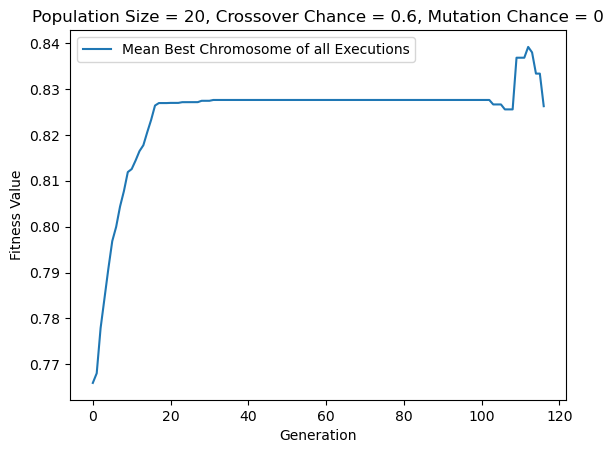
\includegraphics[width=\textwidth]{Figures/1. Means for AA = 1.png}
	\caption{Μέση Καμπύλη για A/A = 1}
\end{figure}

\begin{figure}[H]
	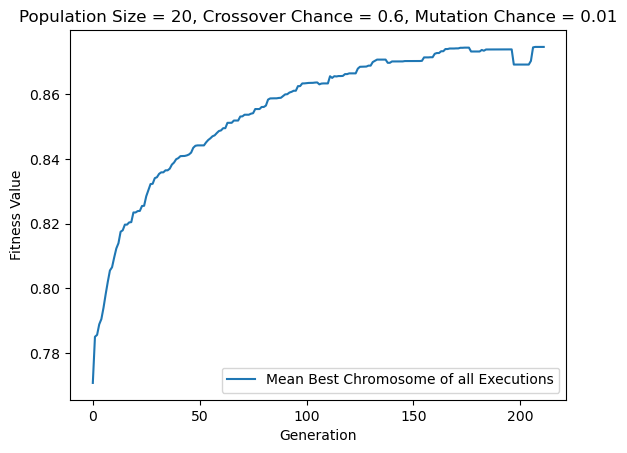
\includegraphics[width=\textwidth]{Figures/3. Means for AA = 2.png}
	\caption{Μέση Καμπύλη για A/A = 2}
\end{figure}

\begin{figure}[H]
	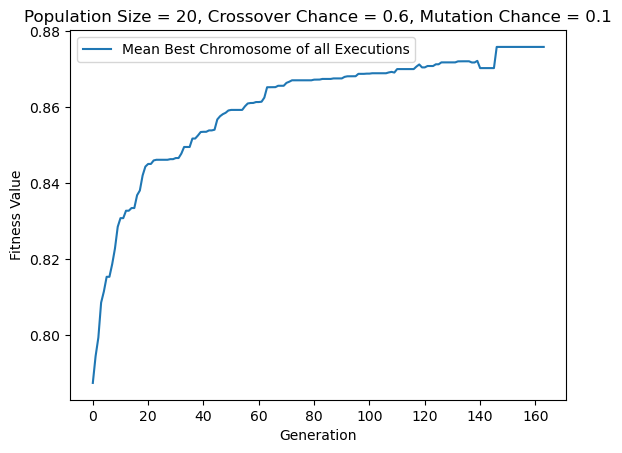
\includegraphics[width=\textwidth]{Figures/5. Means for AA = 3.png}
	\caption{Μέση Καμπύλη για A/A = 3}
\end{figure}

\begin{figure}[H]
	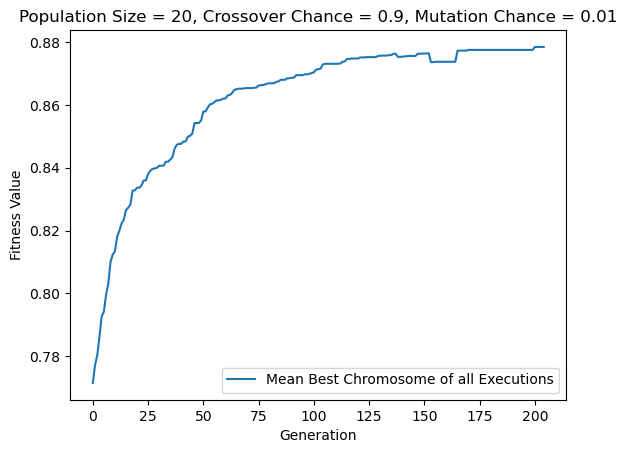
\includegraphics[width=\textwidth]{Figures/7. Means for AA = 4.png}
	\caption{Μέση Καμπύλη για A/A = 4}
\end{figure}

\begin{figure}[H]
	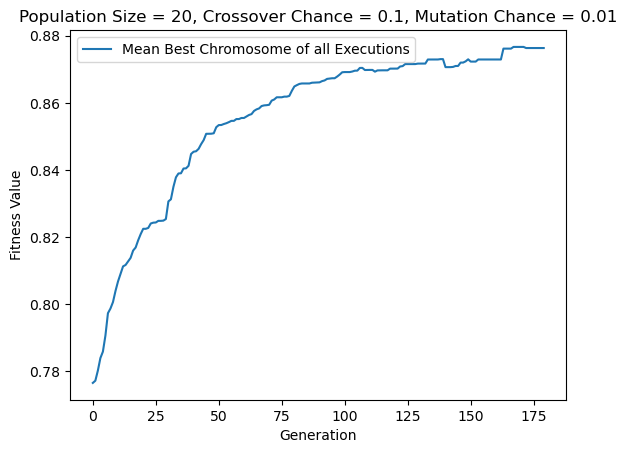
\includegraphics[width=\textwidth]{Figures/9. Means for AA = 5.png}
	\caption{Μέση Καμπύλη για A/A = 5}
\end{figure}

\begin{figure}[H]
	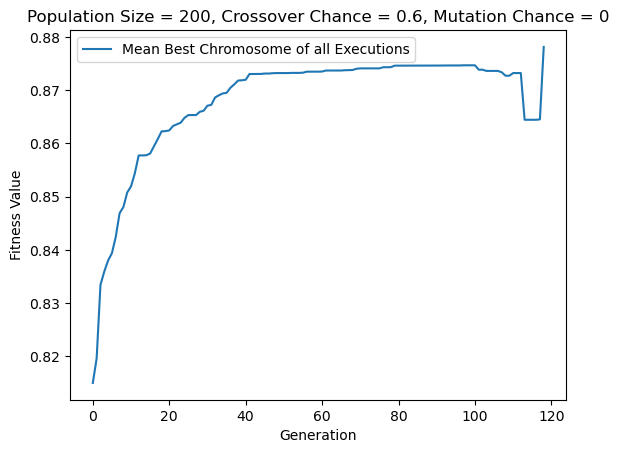
\includegraphics[width=\textwidth]{Figures/11. Means for AA = 6.png}
	\caption{Μέση Καμπύλη για A/A = 6}
\end{figure}

\begin{figure}[H]
	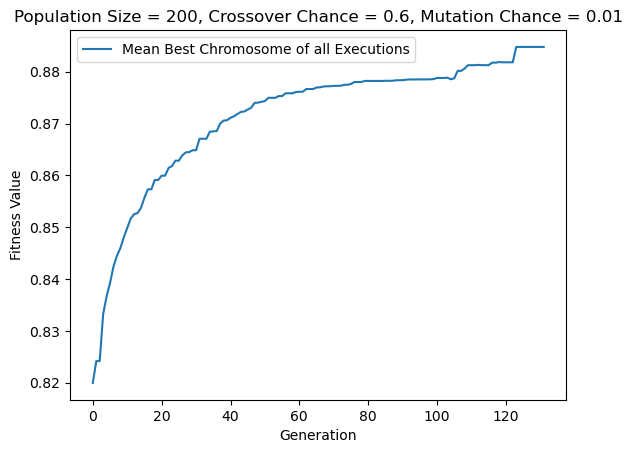
\includegraphics[width=\textwidth]{Figures/13. Means for AA = 7.png}
	\caption{Μέση Καμπύλη για A/A = 7}
\end{figure}

\begin{figure}[H]
	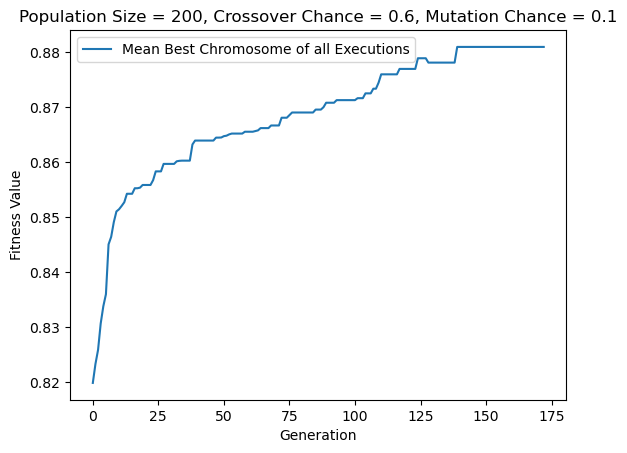
\includegraphics[width=\textwidth]{Figures/15. Means for AA = 8.png}
	\caption{Μέση Καμπύλη για A/A = 8}
\end{figure}

\begin{figure}[H]
	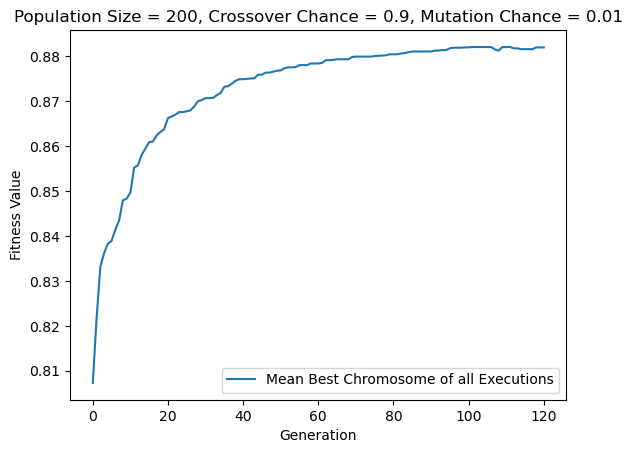
\includegraphics[width=\textwidth]{Figures/17. Means for AA = 9.png}
	\caption{Μέση Καμπύλη για A/A = 9}
\end{figure}

\begin{figure}[H]
	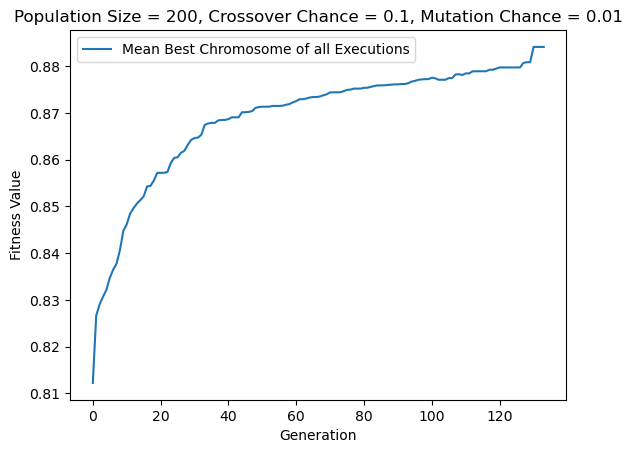
\includegraphics[width=\textwidth]{Figures/19. Means for AA = 10.png}
	\caption{Μέση Καμπύλη για A/A = 10}
\end{figure}


\subsubsection{Καμπύλη κάθε εκτέλεσης ξεχωριστά}
\begin{figure}[H]
	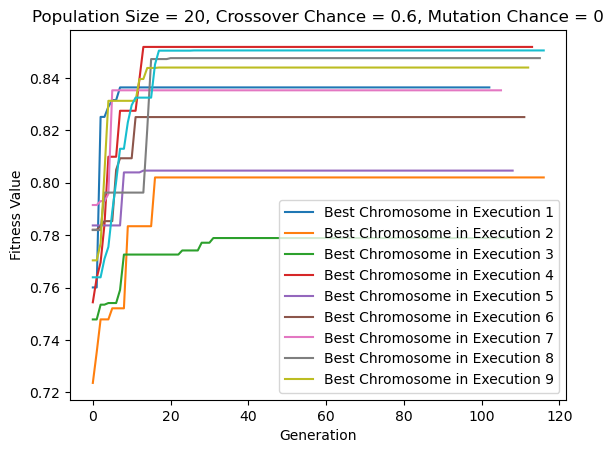
\includegraphics[width=\textwidth]{Figures/2. All for AA = 1.png}
	\caption{Καμπύλη για κάθε εκτέλεση για A/A = 1}
\end{figure}

\begin{figure}[H]
	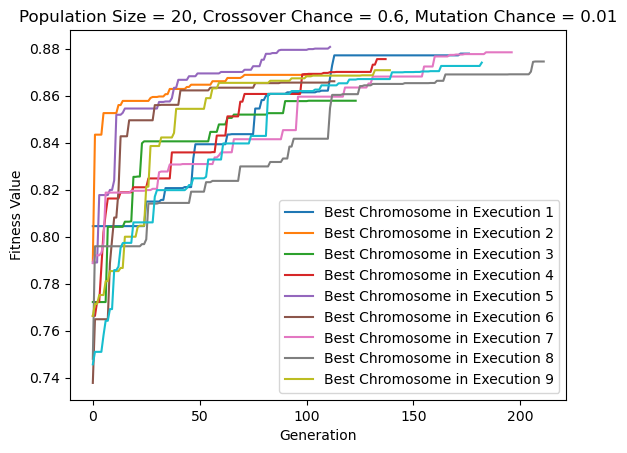
\includegraphics[width=\textwidth]{Figures/4. All for AA = 2.png}
	\caption{Καμπύλη για κάθε εκτέλεση για A/A = 2}
\end{figure}

\begin{figure}[H]
	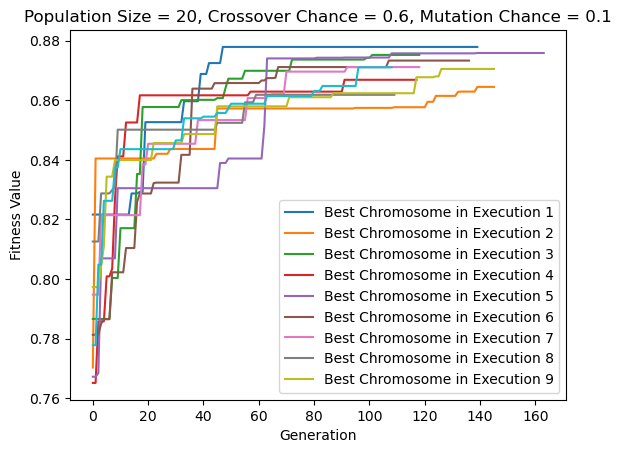
\includegraphics[width=\textwidth]{Figures/6. All for AA = 3.png}
	\caption{Καμπύλη για κάθε εκτέλεση για A/A = 3}
\end{figure}

\begin{figure}[H]
	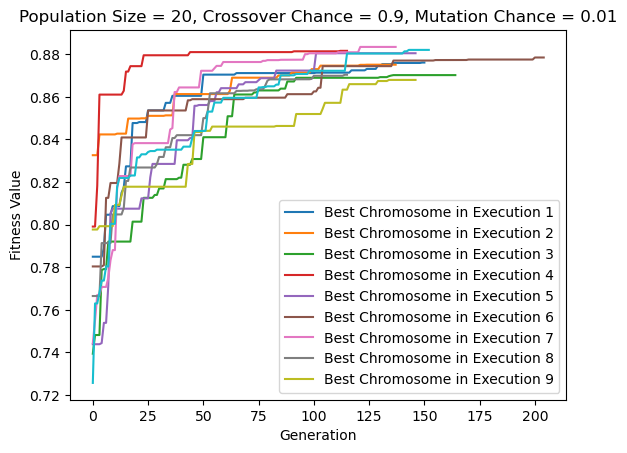
\includegraphics[width=\textwidth]{Figures/8. All for AA = 4.png}
	\caption{Καμπύλη για κάθε εκτέλεση για A/A = 4}
\end{figure}

\begin{figure}[H]
	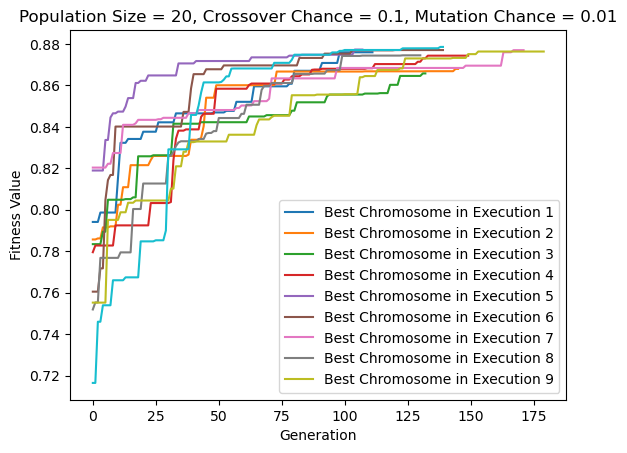
\includegraphics[width=\textwidth]{Figures/10. All for AA = 5.png}
	\caption{Καμπύλη για κάθε εκτέλεση για A/A = 5}
\end{figure}

\begin{figure}[H]
	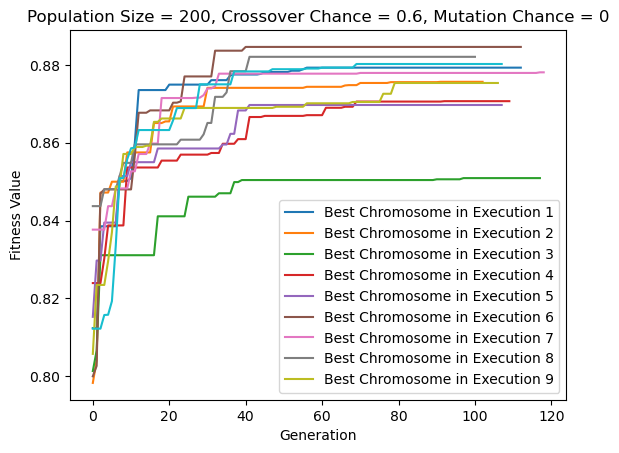
\includegraphics[width=\textwidth]{Figures/12. All for AA = 6.png}
	\caption{Καμπύλη για κάθε εκτέλεση για A/A = 6}
\end{figure}

\begin{figure}[H]
	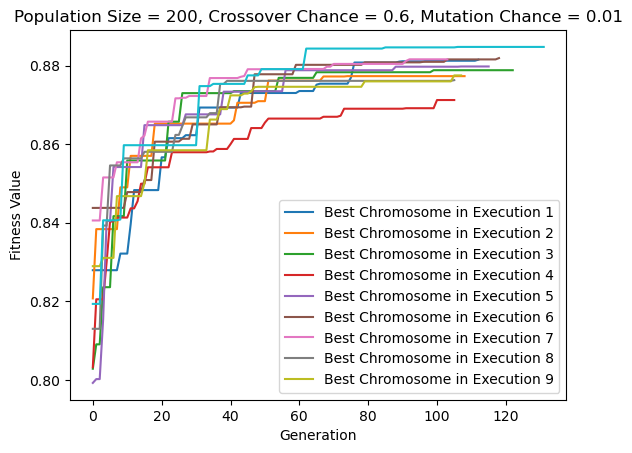
\includegraphics[width=\textwidth]{Figures/14. All for AA = 7.png}
	\caption{Καμπύλη για κάθε εκτέλεση για A/A = 7}
\end{figure}

\begin{figure}[H]
	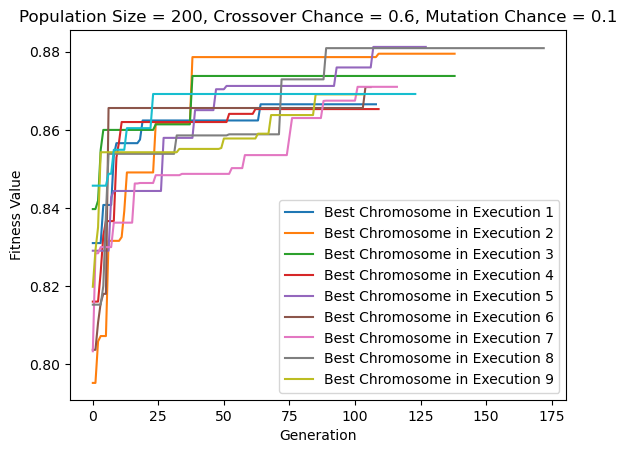
\includegraphics[width=\textwidth]{Figures/16. All for AA = 8.png}
	\caption{Καμπύλη για κάθε εκτέλεση για A/A = 8}
\end{figure}

\begin{figure}[H]
	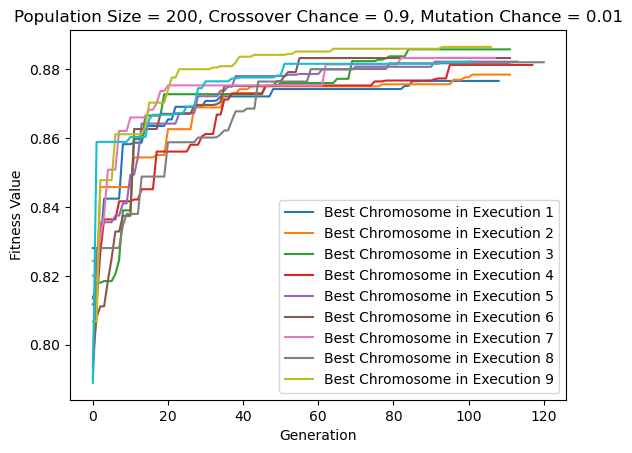
\includegraphics[width=\textwidth]{Figures/18. All for AA = 9.png}
	\caption{Καμπύλη για κάθε εκτέλεση για A/A = 9}
\end{figure}

\begin{figure}[H]
	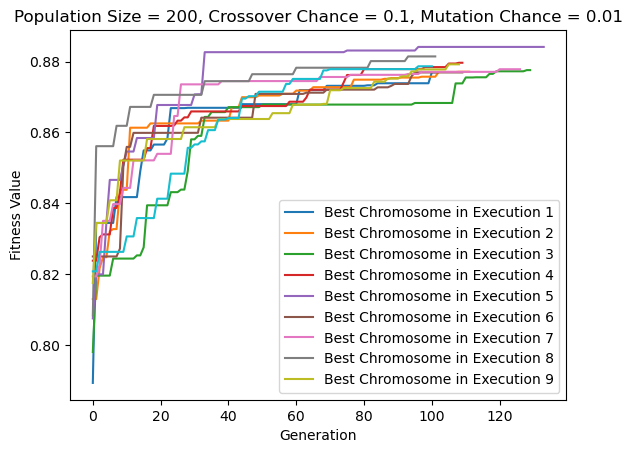
\includegraphics[width=\textwidth]{Figures/20. All for AA = 10.png}
	\caption{Καμπύλη για κάθε εκτέλεση για A/A = 10}
\end{figure}

\subsection{Συμπεράσματα}

\subsubsection{Σχετικά με μέγεθος πληθυσμού}

Σχετικά με το μέγεθος πληθυσμού παρατηρώ αρχικά ότι με τον μεγαλύτερο πληθυσμό χρειάστηκε κατά μέσο όρο μικρότερος αριθμός γενεών ώστε να υπάρξει σύγκλιση. Αυτό είναι επειδή με μεγαλύτερο πληθυσμό τυχαία υπάρχει μεγαλύτερη πιθανότητα να βρεθούν καλές λύσεις, που πιθανότατα να επιλεχτούν για τις επόμενες γενεές, άρα το πρόγραμμα φτάνει γρηγορότερα σε σημείο που συγκλίνει στη βέλτιστη πιθανή λύση.

Σχετικά με τη μέση τιμή fitness δεν παρατηρώ ιδιαίτερη διαφορά σε σχέση με τους μικρότερους πληθυσμούς, επειδή ο αλγόριθμος και στις δύο περιπτώσεις συγκλίνει στη βέλτιστη λύση, απλά στη περίπτωση του μικρότερου πληθυσμού αυτό απαιτεί παραπάνω γενεές.

Στις καμπύλες επίσης η μόνη διαφορά που παρατηρώ για τους διαφορετικούς αριθμούς μεγέθους πληθυσμού είναι ο ρυθμός βελτίωσης, που προκύπτει από τη διαφορά στο συνολικό αριθμό γενεών στον άξονα x, όπως αναφέρθηκε προηγουμένως.

\subsubsection{Σχετικά με πιθανότητα διασταύρωσης}

Σχετικά με τη πιθανότητα διασταύρωσης παρατηρώ ότι οδηγεί συνήθως σε καλύτερες τελικές μέσες τιμές fitness. Αυτό συμβαίνει επειδή με μεγαλύτερη πιθανότητα διασταύρωσης δοκιμάζονται περισσότερες τιμές για τα γονίδια των χρωμοσωμάτων, που οδηγούν σε καλύτερη αναζήτηση των πεδίων των τιμών και τη αυξημένη δυνατότητα για εύρεση των χαρακτηριστικών που οδηγούν στο υψηλό fitness.

Εδώ συμβάλλουν και τα χαρακτηριστικά της διασταύρωσης διπλού σημείου που χρησιμοποίησα, τα χαρακτηριστικά της οποίας εξήγησα σε προηγούμενο ερώτημα.

Κατά τα άλλα ως προς το μέσο αριθμό γενεών (ή τη ταχύτητα σύγκλισης ισοδύναμα στις γραφικές) δεν παρατηρώ διαφορά με διαφορετικές τιμές πιθανότητας διασταύρωσης.

\subsubsection{Σχετικά με πιθανότητα μετάλλαξης}

Σχετικά με τη πιθανότητα μετάλλαξης παρατηρώ στις καμπύλες ανά εκτέλεση ότι όσο πιο μικρή η πιθανότητα τόσο μεγαλύτερη διακύμανση έχουν οι τιμές στις οποίες γίνεται η σύγκλιση. Αυτό συμβαίνει επειδή όσο μικρότερη η πιθανότητα μετάλλαξης, τόσο μικρότερο μέρος του πεδίου αναζήτησης εξερευνιέται και ο γενετικός αλγόριθμος είναι επιρρεπής σε σύγκλιση σε τοπικά ελάχιστα. Οπότε όσο μεγαλύτερη είναι η πιθανότητα μετάλλαξης τόσο πιο ομοιόμορφα είναι τα αποτελέσματα από εκτέλεση σε εκτέλεση, το οποίο είναι επιθυμητό χαρακτηριστικό.

Σημειώνω επίσης ότι υπάρχει μια σχετική αύξηση στις μέσες τιμές fitness από μηδενική μετάλλαξη σε ύπαρξη πιθανότητα μετάλλαξης, επειδή περισσότερες εκτελέσεις φτάνουν πιο κοντά στο ολικό μέγιστο μέσω της καλύτερης αναζήτησης του πεδίου τιμών.

Ακόμα σημειώνω ότι η ταχύτητα σύγκλισης είναι κάπως μεγαλύτερη για μεγάλη πιθανότητα μετάλλαξης (0.1), επειδή υπάρχει ρίσκο να χαθούν τα σωστά patterns στις τιμές που βρέθηκαν μέσω μετάλλαξης, το οποίο βέβαια αντιμετωπίζει και ο ελιτισμός που χρησιμοποιήθηκε.

Τέλος αναφέρω ότι στην απόδοση συνέβαλλε και η επιλογή της τυχαίας μετάλλαξης, την οποία έχω αναλύσει σε προηγούμενο ερώτημα.

\subsection{Είσοδος βέλτιστου στο ΤΝΔ}

\textbf{Σημείωση:} Επειδή δεν επισημαίνεται στην εκφώνηση αν θέλετε να βάλουμε στο ΤΝΔ το βέλτιστο άτομο από όλες τις εκτελέσεις ή το μέσο βέλτιστο άτομο ή το βέλτιστο άτομο για κάθε εκτέλεση για κάθε Α/Α, αποφάσισα να υλοποιήσω τη πρώτη επιλογή που ανέφερα, ώστε να μην εμφανίζω υπερβολικά πολλά δεδομένα, παρόλα αυτά στον κώδικά μου βλέπω τη κλάση για κάθε εκτέλεση και λαμβάνω και αυτές τις πληροφορίες υπόψη μου για την εξαγωγή των συμπερασμάτων.

Αναφέρω επίσης ότι πολλές φορές το βέλτιστο άτομο με τη μεγαλύτερη καταλληλότητα από όλες τις εκτελέσεις δεν είχε τη μεγαλύτερη πιθανότητα από όλα τα βέλτιστα άτομα όλων των εκτελέσεων, παρόλα αυτά σε κάθε περίπτωση όλα τα βέλτιστα άτομα ανήκαν στη τελική στη κλάση 'sitting' (ένας ακόμα λόγος που αναφέρω μόνο τη βέλτιστη λύση όλων των εκτελέσεων).

\subsubsection{Αποτελέσματα ΤΝΔ ανά Α/Α}


\begin{enumerate}
    \item Ποσοστό για κλάση 'sitting': 0.9978862404823303

          Επιλεγμένη κλάση: 'sitting'
    \item Ποσοστό για κλάση 'sitting': 0.7064703106880188

          Επιλεγμένη κλάση: 'sitting'
    \item Ποσοστό για κλάση 'sitting': 0.9918357133865356

          Επιλεγμένη κλάση: 'sitting'
    \item Ποσοστό για κλάση 'sitting': 0.9976669549942017

          Επιλεγμένη κλάση: 'sitting'
    \item Ποσοστό για κλάση 'sitting': 0.9930181503295898

          Επιλεγμένη κλάση: 'sitting'
    \item Ποσοστό για κλάση 'sitting': 0.792059600353241

          Επιλεγμένη κλάση: 'sitting'
    \item Ποσοστό για κλάση 'sitting': 0.999914288520813

          Επιλεγμένη κλάση: 'sitting'
    \item Ποσοστό για κλάση 'sitting': 0.9999469518661499

          Επιλεγμένη κλάση: 'sitting'
    \item Ποσοστό για κλάση 'sitting': 0.9946921467781067

          Επιλεγμένη κλάση: 'sitting'
    \item Ποσοστό για κλάση 'sitting': 0.9999961853027344

          Επιλεγμένη κλάση: 'sitting'
\end{enumerate}

\subsubsection{Συμπεράσματα}

Από τα αποτελέσματα της εισαγωγής των καλυτέρων από όλες τις εκτελέσεις για όλες τις περιπτώσεις συμπεραίνω πως σε κάθε περίπτωση η κλάση που βρέθηκε ήταν η σωστή. Αυτό συμβαίνει επειδή, όπως φαίνεται και στα αποτελέσματα των παραπάνω ερωτημάτων, όλες οι περιπτώσεις και εκτελέσεις συγκλίνουν σε ικανοποιητικό βαθμό στις βέλτιστες λύσεις.

Επίσης σημειώνω ότι το πρόβλημα εκ φύσεως, ως πρόβλημα κατηγοριοποίησης είναι ανθεκτικό σε μικρά σφάλματα, εφόσον απαιτείται μόνο το ποσοστό για τη κλάση 'sitting' να το μεγαλύτερο για να επιλεχθεί η κλάση αυτή.

Τέλος σημειώνω ότι στα παραπάνω αποτελέσματα, οι διαφορές στα ποσοστά για τη κλάση 'sitting' των καλυτέρων κάθε περίπτωση ήταν επιρρεπής σε κάποια τυχαιότητα, και πολλές φορές άλλες τιμές που δεν ήταν οι βέλτιστες όλων των εκτελέσεων είχαν μεγαλύτερα ποσοστά. Αυτό συμβαίνει επειδή δεν υπάρχει ένα προς ένα αντιστοίχηση με τις τιμές του fitness function για τον γενετικό αλγόριθμο και τη λειτουργία του νευρωνικού δικτύου για τον υπολογισμό των ποσοστών, οπότε ενώ οι κατηγοριοποιήσεις γίνονται πάντα σωστά και τα ποσοστά για τη σωστή κατηγοριοποίηση είναι υψηλά, υπάρχει μια διακύμανση στα ποσοστά λόγω τυχαιότητας.

\end{document}
